\section{Evaluation} \label{evaluation}

Die Bearbeitung der Forschungsfrage hat folgende Ergebnisse hervorgebracht: Aus ursprünglich 96~924 potenziell relevanten Ufo-Sichtungen im Datensatz konnten für 2~020 Sichtungen zu dem Zeitpunkt passende Wetterdaten gefunden werden, das entspricht ungefähr 2,1\%. Mit welcher Art der drei Vergleichsdaten die Sichtungen analysiert wurden lässt sich in Tabelle \ref{tab:data} ablesen.

\begin{figure}[t]
    \centering
    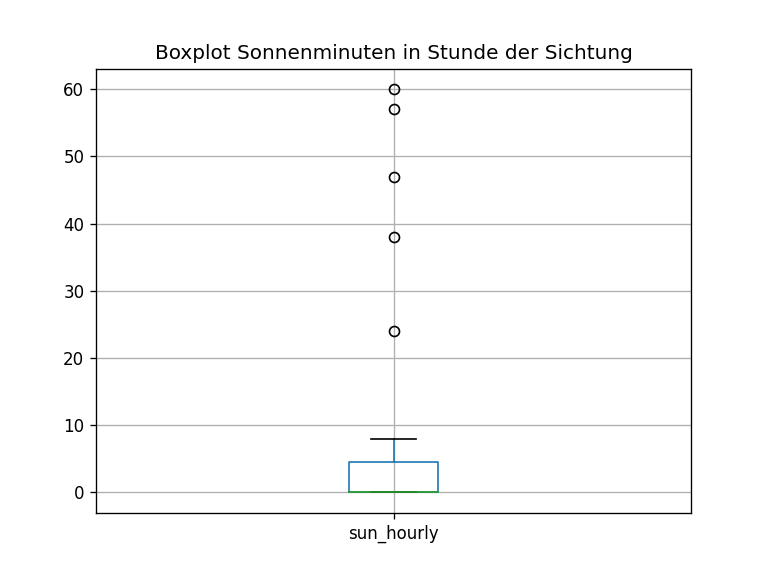
\includegraphics[width=\columnwidth]{hourly_suntime_boxplot}
    \caption{Sonnenminuten pro Stunde.}
    \label{fig:hourly_suntime}
\end{figure}

Die Vergleichsdaten mit dem am Abstand wenigsten Vorkommen bilden die Sonnenminuten pro Stunde mit lediglich 26 Einträgen. Wie in Abbildung \ref{fig:hourly_suntime} zu erkennen ist, befindet sich die Mehrheit davon im Bereich von 0 bis 5 Sonnenminuten pro Stunde. Vereinzelte Ausreißer reichen gegen 50 bis 60 Sonnenminuten. 

\begin{figure}[t]
    \centering
    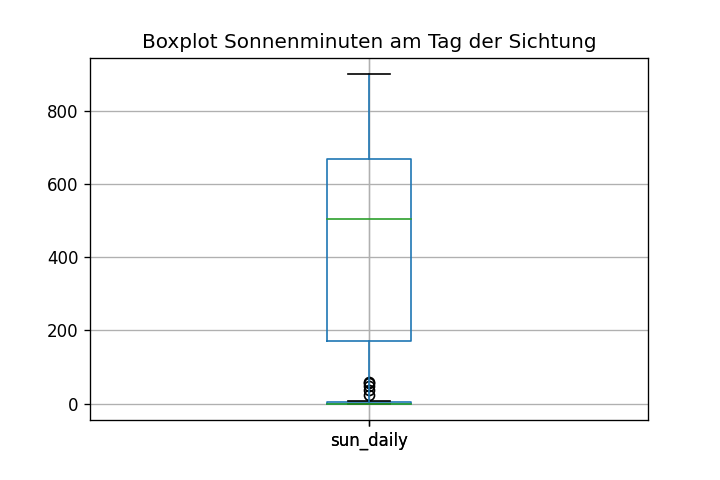
\includegraphics[width=\columnwidth]{daily_suntime_boxplot}
    \caption{Sonnenminuten pro Tag.}
    \label{fig:daily_suntime}
\end{figure}

Abbildung \ref{fig:daily_suntime} beschreibt die Verteilung der Sonnenminuten pro Tag an jeder verfügbaren Ufo-Sichtung. Die mittleren 50\% der Ergebnisse sind hierbei, im Gegensatz zu den stündlichen Sonnenminuten, breiter verteilt. Sie reichen von 200 bis 700 Sonnenminuten pro Tag mit wenigen Ausreißern, welche nur gegen weniger Minuten streben. Im Schnitt scheint die Sonne während eines Tages, an dem ein vermeintliches Ufo gesichtet wurde, um die 500 Minuten -- also etwas mehr als 8 Stunden. In Anbetracht dessen, dass die durchschnittlichen Sonnenstunden in den USA im Bereich zwischen 2 Stunden im Winter und bis zu 12 Stunden im Sommer reichen, kann man den Ufo-Sichtungen eine leichte Überdurchschnittlichkeit an Sonnenstunden während eines Sichtungstages zuordnen\cite{statista:2021}.

Das Attribut mit den am meisten verwendbaren Vergleichsdaten bilden die Condition Codes mit 1~886 Daten zur entsprechenden Sichtung. Auf ihnen liegt in dieser Evaluation das Hauptaugenmerk und die beiden Attribute der Sonnenminuten ergänzen diese. Aus Abbildung \ref{fig:coco_pie} geht hervor, dass sechs der 17 ermittelten Condition Codes überwiegen. Schönwetter \enquote{Fair} dominiert die absolute Häufigkeit an Einheiten mit einer Anzahl von 603. Die genauen Werte können der Tabelle \ref{tab:coco} entnommen werden. Im folgenden Abschnitt werden lediglich die sechs Attribute mit der größten Ausprägung (Codes 1, 2, 3, 4, 5, 7). Zusammengerechnet umfassen diese Condition Code-Gruppen 1~691 aller Ufo-Sichtungen -- das entspricht 89,7\%. Diese Codes können weiter in zwei Gruppen eingeteilt werden: Zum Ersten \enquote{gutes Wetter} mit \enquote{Clear}, \enquote{Fair} und \enquote{Cloudy} und zum Weitern \enquote{schlechtes Wetter} mit \enquote{Overcast}, \enquote{Fog} und \enquote{Light Rain}. Die Bezeichnungen können \cite{coco:2021} entnommen werden. Damit die Gruppe \enquote{gutes Wetter} auf 1~193 Einheiten und die Gruppe \enquote{schlechtes Wetter} auf 498 Einheiten. Die restlichen nicht in Gruppen eingeteilten Codes umfassen vor allem weitere Stufen von Regen- und Schneeschauern sowie Gewitter. Generell kann man sagen, dass je höher der Condition Code ist, desto \enquote{schlechter} ist das Wetter und umso schlechter kann man Objekte am Himmel erkennen. Die Codes sind also ordinal skaliert mit einem Median von $\tilde{x}$ = 3. Ausgehend vom Median, welcher sich innerhalb der Gruppe \enquote{gutes Wetter} befindet, gibt es überdurchschnittlich mehr Sichtungen mit gutem als mit schlechtem Wetter.

Diese Werte lassen sich wie folgt interspretieren: Zum einen ist es ersichtlich, dass es bei gutem Wetter und freiem Himmel mehr Möglichkeiten gibt, Flugobjekte zu entdecken. Dies würde die Dominanz der Gruppe \enquote{gutes Wetter} erklären. Es erweckt allerdings auch den Gedanken, wieso es bei vermeintlich schlechterem Wetter, im Vergleich zu den nicht in Gruppen eingeteilten Condition Codes, ebenso eine höhere Anzahl an Sichtungen gab. Zum anderen lassen sich unter den nicht Guppoerten Codes drei Ausreißer entdecken: \enquote{Light Snowfall}, \enquote{Heavy Rain Shower} und \enquote{Thunderstorm}. Ihre vergleichsweise häufigen Eintritte im Bereich der nicht gruppierten Codes lassen sich entweder durch eine vergleichsweise höhere Eintrittswahrscheinlichkeit dieser Ereignisse in der Natur, oder durch diese Ereignisse ausgelösten schlechte Sichtverhältnisse und die damit verbundene Möglichkeit, dass Signale und Lichte fehlinterpretiert werden, beschreiben. Letzteres bleibt allerdings nur eine Vermutung, da diese Theorie durch das geringere Auftreten einer Ufo-Sichtung während \enquote{Heavy Snowfall} und \enquote{Storm} im Gegensatz zu ihren einfacheren Varianten \enquote{Light Snowfall} und \enquote{Thunderstorm} widerlegt wurde, denn durch die Verstärkung von Schneefall oder Sturm verschlechtern sich allgemein die Sichtverhältnisse und erhöhen die Wahrscheinlichkeit von Fehlinterpretationen.

Wir halten fest: je \enquote{besser} das Wetter ist, desto wahrscheinlicher ist es, dass ein vermeintliches Ufo gesichtet wird. Die überdurchschnittlichen Sonnenminuten an einem Tag einer Ufo-Sichtung unterstreicht diese Erkenntnis.

\begin{table}[t]
    \caption{Condition Codes.}
    \label{tab:coco}
    \centering
    \small
    \begin{tabular}{l l r}
        \toprule
        Code & Weather Condition\cite{coco:2021} & Anzahl\\
        \midrule
        0 & - & 15\\
        1 & Clear & 227\\
        2 & Fair & 603\\
        3 & Cloudy & 363\\
        4 & Overcast & 93\\
        5 & Fog & 186\\
        7 & Light Rain & 219\\
        8 & Rain & 51\\
        9 & Heavy Rain & 9\\
        12 & Sleet & 1\\
        14 & Light Snowfall & 42\\
        15 & Snowfall & 2\\
        16 & Heavy Snowfall & 1\\
        17 & Rain Shower & 9\\
        18 & Heavy Rain Shower & 23\\
        25 & Thunderstorm & 35\\
        26 & Heavy Thunderstorm & 5\\
        27 & Storm & 2\\
        \bottomrule
    \end{tabular}
\end{table}
